\documentclass[a4paper,12pt,titlepage]{report}
\usepackage{titling}
\usepackage{amsmath,amssymb}
\usepackage{graphicx}
\usepackage{hyperref}
\usepackage[left=20mm,right=20mm,top=15mm,bottom=15mm]{geometry}
\usepackage{caption}
\usepackage{siunitx} % For clean units formatting
\usepackage{appendix}
\usepackage{titlepic}
\usepackage{ragged2e}

\usepackage[backend=biber]{biblatex}
\addbibresource{references.bib}

\usepackage{chngcntr}
\counterwithout{figure}{chapter}
\counterwithout{table}{chapter}
\counterwithout{equation}{chapter}

\usepackage{listings}
\usepackage{xcolor}

\counterwithout{figure}{chapter}
\counterwithout{table}{chapter}
\counterwithout{equation}{chapter}

% --- Title Info ---
\title{EE475 - ORBITS Design}
\author{Scott McBride --- 202215222}
\titlepic{
\includegraphics[width=0.9\textwidth]{./Images/ORBITS_Logo.png}}
\date{\today}

\begin{document}
\begin{titlepage}
    \begin{center}
        \vspace*{3cm}
        \begin{minipage}{0.8\textwidth}
            \justifying
            \noindent \color{gray}
            I hereby declare that this work has not been submitted for any other degree/course at this University or any other institution and that, except where reference is made to the work of other authors, the material presented is original and entirely the result of my own work at the University of Strathclyde under the supervision of Dr Astrid A Werkmeister.”
        \end{minipage}
        \vfill
        \Huge
        \textbf{ORBITS}
            
        \vspace{0.5cm}
        \LARGE
        Outreach and Research Build for Interactively Teaching Satellites
            
        \vspace{1.5cm}
            
        \begin{figure}[!h]
            \centering
            \begin{minipage}{0.4\textwidth}
                \centering
                
\includegraphics[width=1\textwidth]{./Images/ORBITS_Logo.png}
            \end{minipage}
            \begin{minipage}{0.4\textwidth}
                \centering
                
\includegraphics[width= 1\textwidth]{./Images/strath_main.jpg}
            \end{minipage}
        \end{figure}  

        \textbf{Scott McBride} \\
        Dr Astrid A Werkmeister\\

        \vspace{0.8cm}
            
        \Large
        Department of Electronic and Electrical Engineering\\
        University of Strathclyde\\
        \today
            
    \end{center}
\end{titlepage}
\tableofcontents
\chapter{Abstract}
The Outreach and Research Build for Interactively Teaching Satellites, referred to as ORBITS herein, is a emulation system for a 1U CubeSat ecosystem including both a ground communication station and a physical ORBITS unit that provides a learning environment for both software and hardware concepts.

The ORBITS project is looking to develop a class based learning material that pupils, students, teachers and lecturers are able to gain hands on experience with to experiment, learn and research into CubeSat development. The ORBITS system looks to have modularity at the forefront of its design, allowing users to create thier own payloads to interact with a stock unit to learn about different aspects of a CubeSat system and development. The system looks to be comprised of Commercial Off The Shelf (COTS) components where possible to keep costs low and allow for easy replacement of faulty parts.

Where applicable SysML diagrams have been used to represent the design of the ORBITS system to describe and provide an alternative method of understanding for users to reference.

\chapter{Introduction}
\section{}

\chapter{Review of Related Work}

\chapter{Design}
\section{Hardware Overview}

The system has been developed using a top down approach starting with the high level requirements and breaking these down into smaller subsystems. Shown within Figure \ref{fig:ORBITS_Requirements} are the high level system requirements for the ORBITS system.

\begin{figure}[h]
    \centering
    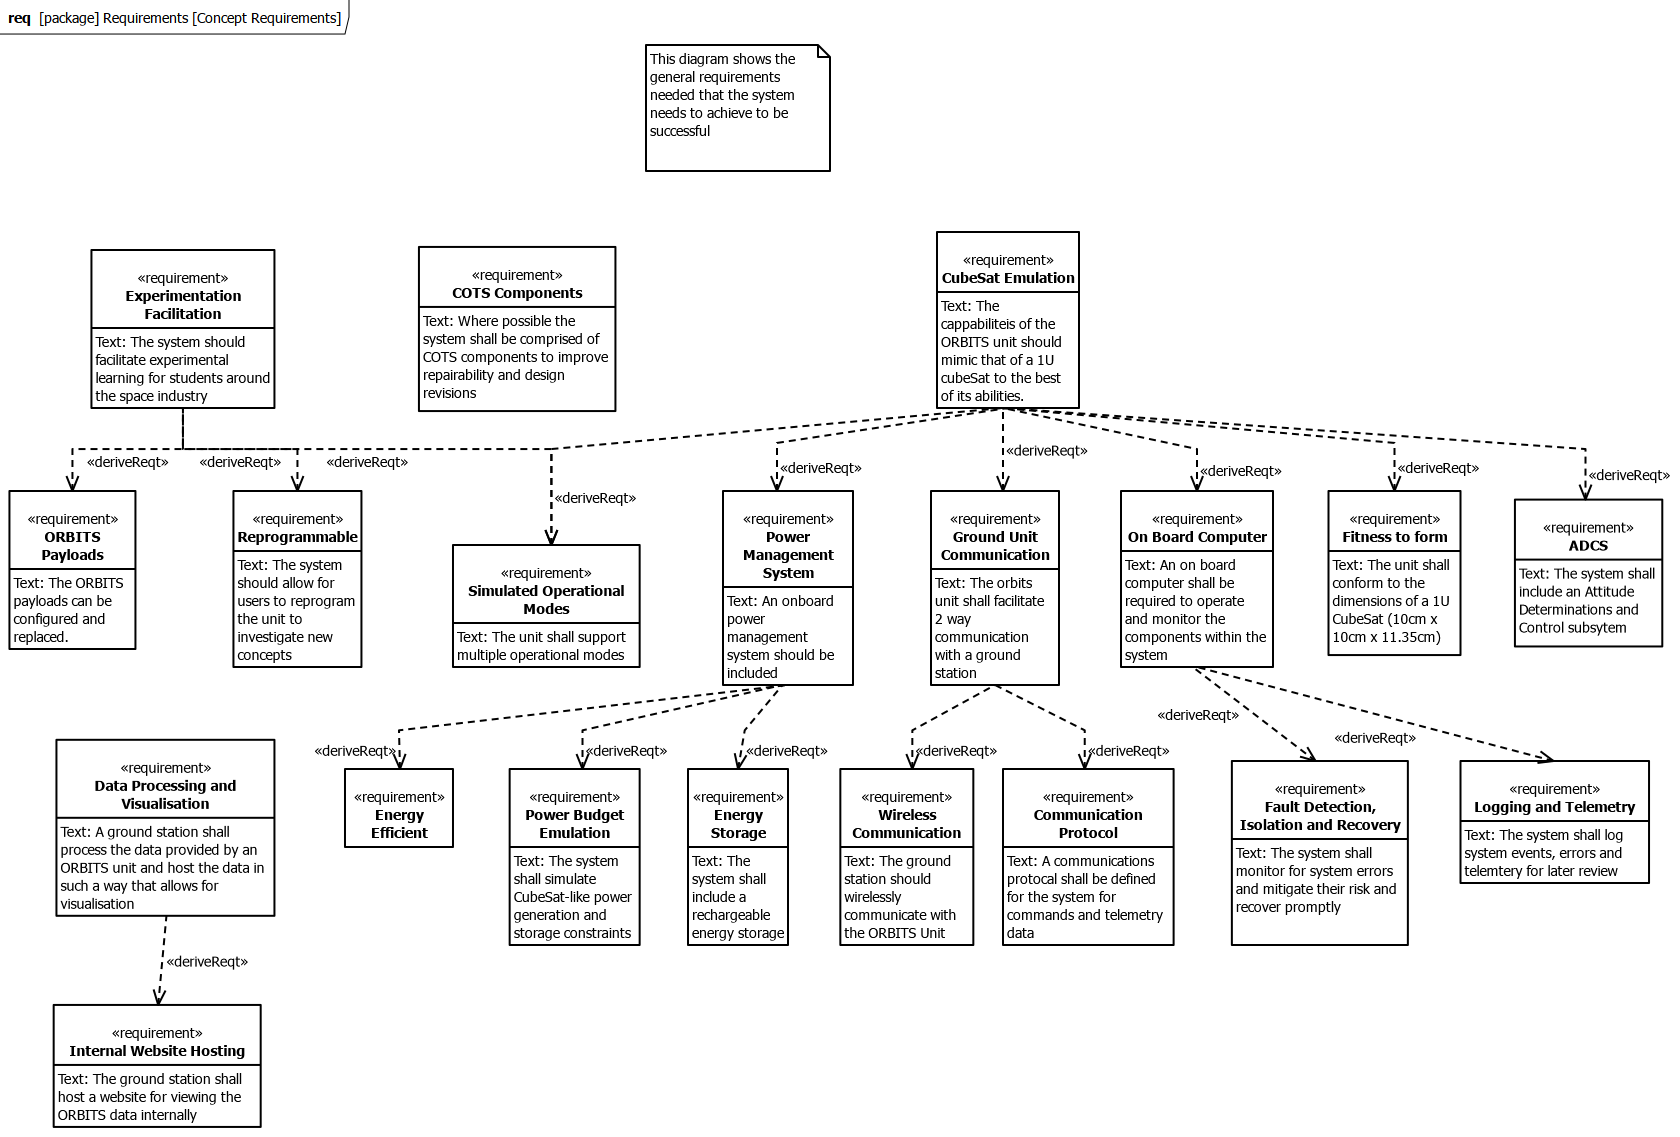
\includegraphics[width=1\textwidth]{./Images/ORBITS_Requirements.png}
    \caption{High Level ORBITS System Requirements}
    \label{fig:ORBITS_Requirements}
\end{figure}

These requirements have been refined through several iterative rounds all looking to provide some atomic metric that the system needs to achieve to be successful and set itself apart from other products currently available on the market.

The main subsystems of the ORBITS system can then be derived from these requirements. These subsystems are listed below:
\begin{itemize}
    \item On-Board Computer (OBC)
    \item Power Management and Distribution Subsystem (PMAD)
    \item Communications Subystem
    \item Attitude Determination and Control Subsystem (ADCS)
    \item Payload
    \item Platform Structure
    \item Ground Station
\end{itemize}

To visualize this breakdown a SysML Block Definition Diagram (BDD) has been created, shown in Figure \ref{fig:ORBITS_BDD}.
\begin{figure}[h]
    \centering
    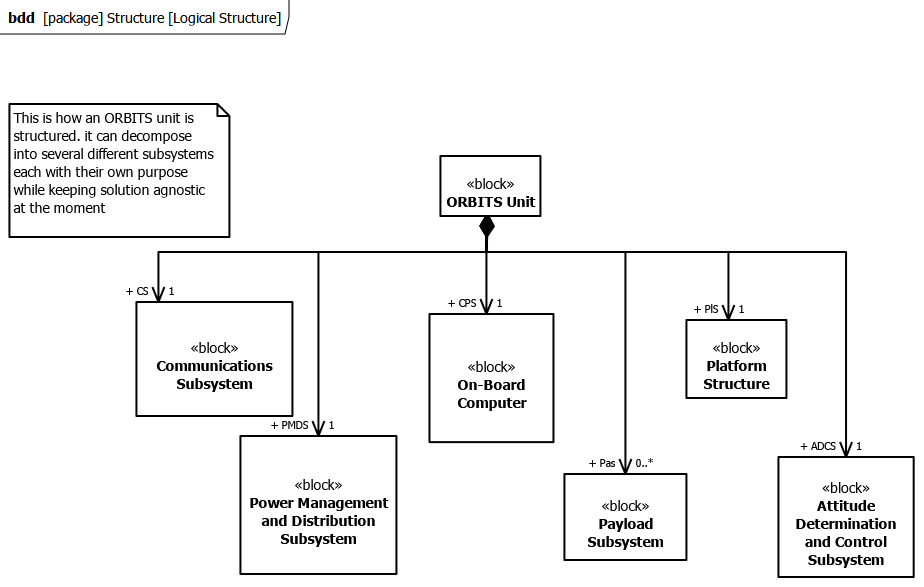
\includegraphics[width=1\textwidth]{./Images/ORBITS_Logical_Structure.png}
    \caption{ORBITS Unit System Block Definition Diagram}
    \label{fig:ORBITS_BDD}
\end{figure}

How each of these subsystems interact with each other is shown in the Internal Block Diagram (IBD) in Figure \ref{fig:ORBITS_IBD}.
\begin{figure}[h]
    \centering
    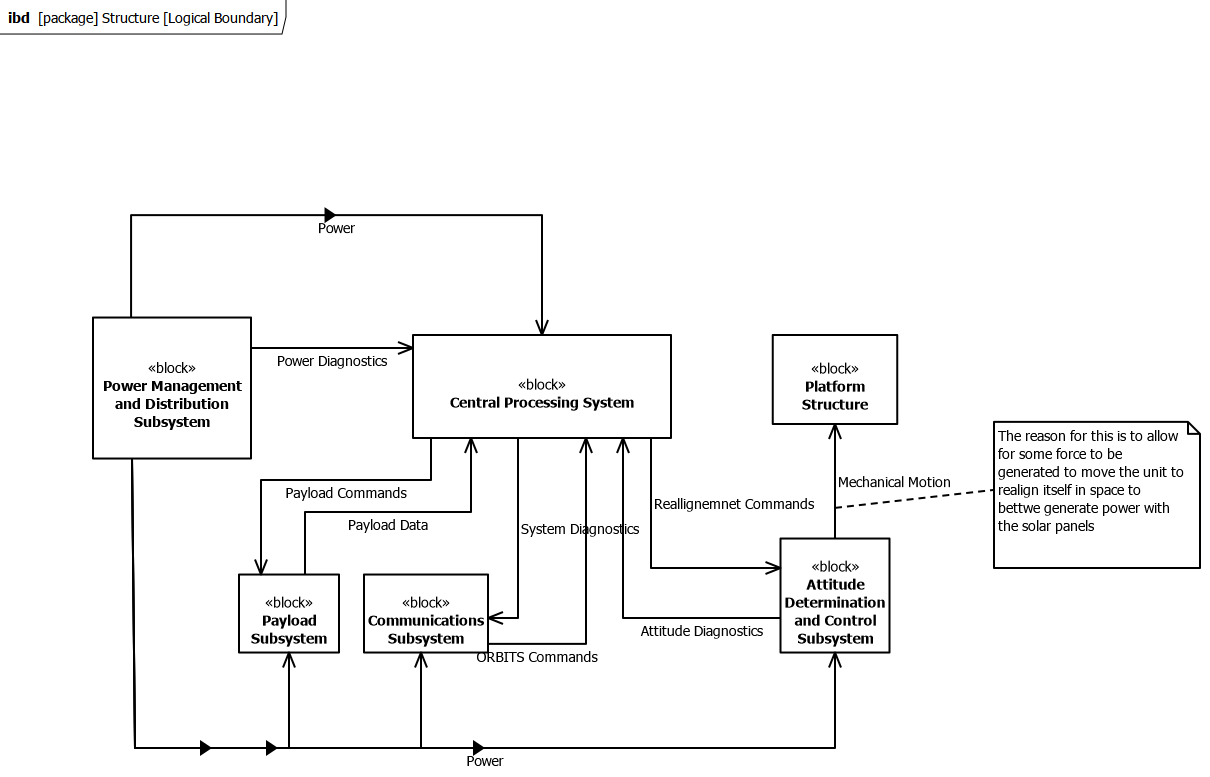
\includegraphics[width=1\textwidth]{./Images/ORBITS_Logical_Boundary.png}
    \caption{ORBITS Unit System Internal Block Diagram}
    \label{fig:ORBITS_IBD}
\end{figure}
Defining the system in this way creates a clear structure as to how the dedicated ORBITS unit should behave allowing for easier development of each subsystem while ensuring that relevant learning materials are able to be created covering each aspect of the system.

\smallskip
the ground station is its own device that provides connectivity to the ORBITS unit from any standard laptop or desktop environment allowing for the development of software and learning materials to be as accessible as possible. 


\section{Hardware Selection and Subsystem Design}
Taking these general design choices into account, each subsystem has been researched and designed to meet the overall system requirements. Each subsystem design is outlined in the following sections. Each section, where relevant had considered multiple options and comparing against several categories. These categories include:
\begin{itemize}
    \item Cost: The monetary cost of the component or subsystem.
    \item Ecosystem: The availability of learning materials, documentation and community support for the component or subsystem.
    \item Performance: The performance of the component or subsystem in terms of its capabilities and specifications.
    \item Price to Performance: The ratio of the cost to the performance of the component or subsystem.
    \item Availability: The availability of the component or subsystem in the market.
\end{itemize}
The components listed within each subsystem are those that were the best fit from these categories resulting in their selection for the ORBITS project.

\subsection{Ground Station}
The ground station is the interface between the user and the ORBITS unit. It provides a platform for users to develop software and interact with the ORBITS unit. The ground station needs to be as accessible as possible for a wide range of different users including pupils, students, teachers and lecturers. To achieve this the ground station should be an add on device with connectivity to any standard laptop or desktop environment. Shown below in Table \ref{tab:ground_station_selected_components} are the selected components for the ground station subsystem.
\begin{table}[h]
    \centering
    \caption{Selected components for the Ground Station}
    \label{tab:ground_station_selected_components}
    \begin{tabular}{|p{4cm}|p{4cm}|p{6cm}|}
    \hline
    \textbf{Component} & \textbf{Part Number} & \textbf{Key Specifications} \\ \hline
    Ground Station & Raspberry Pi Zero 2 W & 1~GHz ARM Cortex-A53, 512~MB SDRAM, 2~W active load \\ \hline
    Communication Module & NRF24L01+ & 2.4~GHz RF band, 250~kbps data rate \\ \hline
    Housing & 3DRPiHousing & Open-source 3D print~\cite{GroundStationCase} \\ \hline
    \end{tabular}
\end{table}

For the communications of the system more context will be provided in the communications subsystem section \ref{communications_subsystem}.

\smallskip
Shown below in Table \ref{tab:ground_station_selection_matrix} is the major component selection for the main ground station computer. 

\begin{table}[h]
\centering
\caption{Ground Station Selection Matrix}
\label{tab:ground_station_selection_matrix}
\begin{tabular}{|p{3cm}|c|c|c|c|c|p{2.5cm}|}
\hline
\textbf{Option} & \textbf{Cost} & \textbf{Ecosystem} & \textbf{Performance} & \textbf{Avail.} & \textbf{P/P} & \textbf{Decision} \\ \hline
Raspberry Pi Zero 2 W & 10 & 8 & 5 & 8 & 10 & Selected \\ \hline
K2B Allwinner H618 & 5 & 3 & 5 & 7 & 5 & Rejected \\ \hline
Orange Pi Zero 2 W & 7 & 6 & 6 & 7 & 7 & Rejected \\ \hline
\end{tabular}
\end{table}

Even though the Raspberry Pi Zero 2 W is not the most powerful option available it was selected for its low cost, large ecosystem and high price to performance ratio in comparison to the other options. The availability of the Raspberry Pi Zero 2 W is also very high with the device being available from a wide range of retailers and distributors while being at a price point that helps minimise the overall cost of an ORBITS kit.

\smallskip

Due to the nature of the Raspberry Pi being a fully featured single board computer it allows for the hosting of all the relevant materials needed for the ORBITS system including compiling user generated software. 

\begin{itemize}
    \item \textbf{Electrical interface:} 5~V input, 2~A max current, overcurrent protection.
    \item \textbf{Data interface:} USB 2.0 (480~Mbps), 2.4GHz 802.11 wireless LAN, Bluetooth LE 4.2.
    \item \textbf{Mechanical interface:} 30 mm x 65 mm board, 4 mounting holes, micro-USB power and data port.
    \item \textbf{Software interface:} Raspberry Pi OS (Linux - Headless Config), USB Gadget mode for host connectivity.
\end{itemize}

With any of the devices needed to operate the ORBITS unit there are some risks that need to be considered. Shown in Table \ref{tab:ground_station_risks} are some of the risks associated with the ground station and their corresponding mitigations.

\begin{table}[h]
\centering
\caption{Risks for the Ground Station}
\label{tab:ground_station_risks}
\begin{tabular}{|p{5cm}|p{2cm}|p{2cm}|p{6cm}|}
\hline
\textbf{Risk} & \textbf{Impact} & \textbf{Likelihood} & \textbf{Mitigation} \\ \hline
Insufficient Device Memory & M & L & Offload memory intense tasks to development machine with static website  \\ \hline
Supply Chain Demand & H & L & Secure a unit for prototype development \\ \hline

\end{tabular}
\end{table}

\subsubsection{Summary}

To allow for the software and development environment to be as accessible as possible the ground station had been selected to interface with any standard laptop or desktop environment. To provide the maximal flexibility the Raspberry Pi Zero 2 W was selected as the ground station. The Raspberry Pi Zero 2 W is a low cost, low power single board computer that provides a wide range of connectivity options including WiFi and Bluetooth shown in figure~\ref{fig:PiZero2W}. The Raspberry Pi Zero 2 W also has a large community and ecosystem of learning materials and documentation which makes it an ideal choice for the ground station.
\begin{figure}[h]
    \centering
    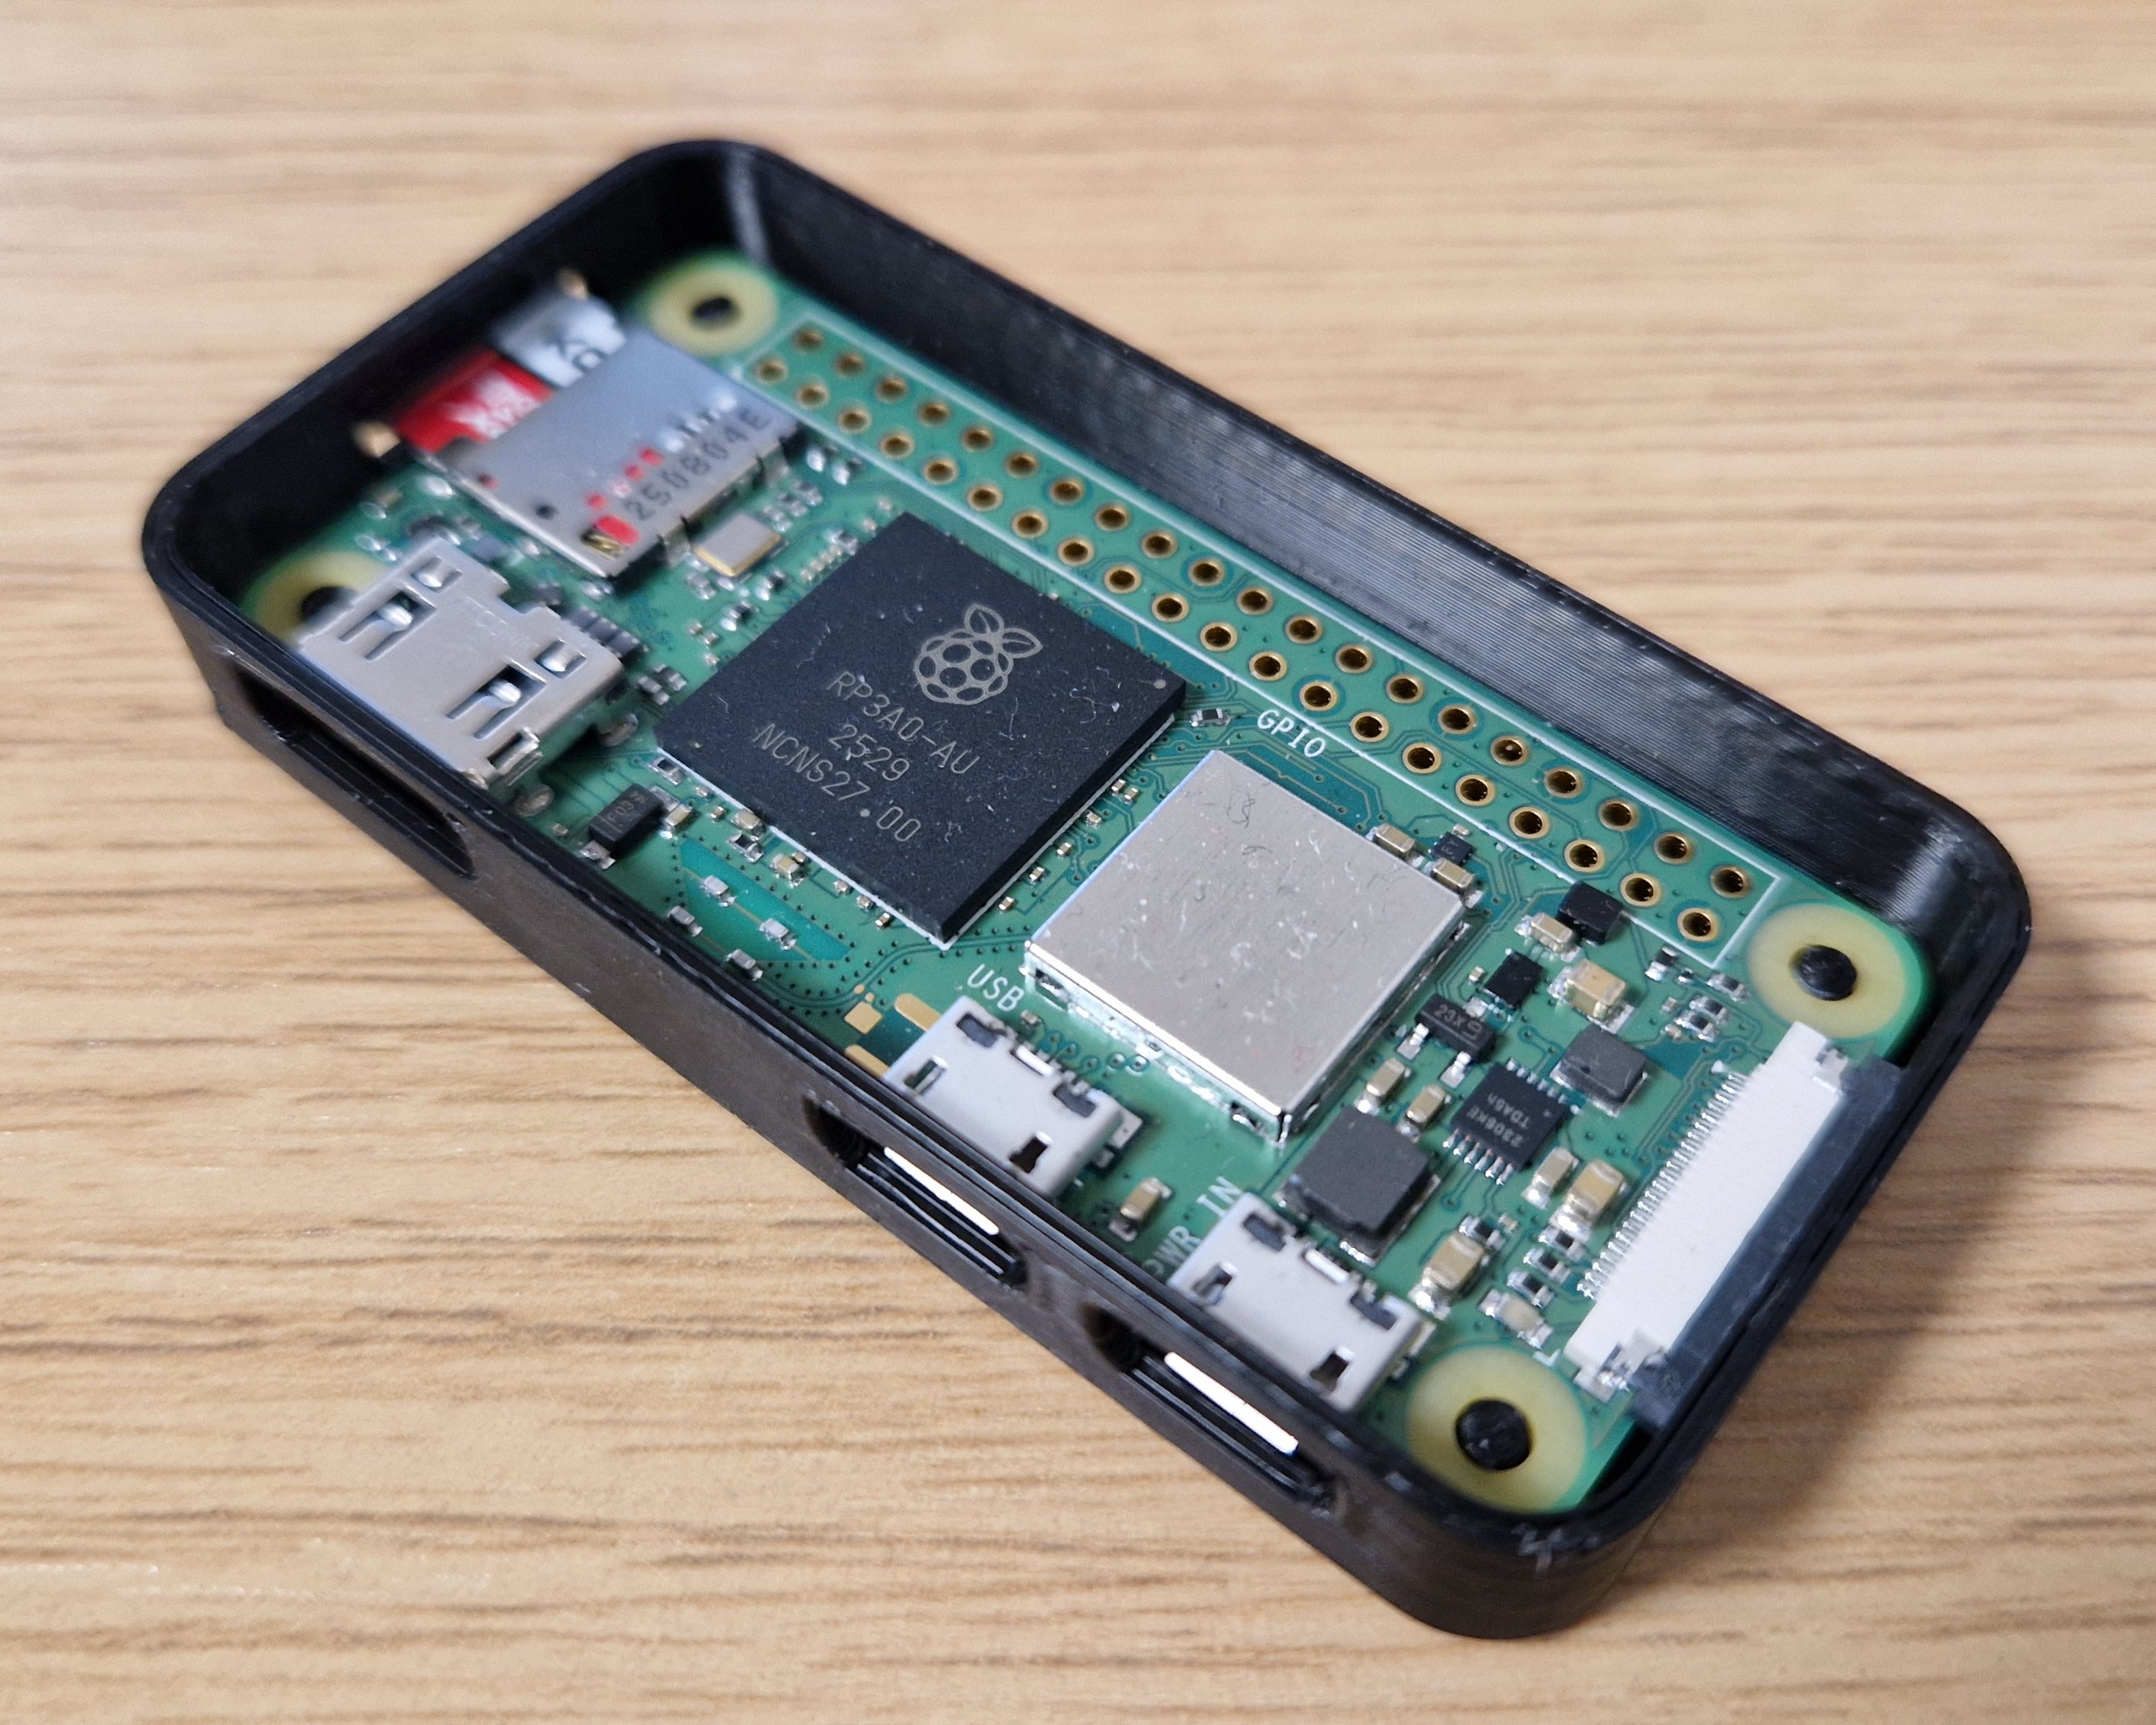
\includegraphics[width=0.5\textwidth]{./Images/PiZero2W.jpg}
    \caption{Raspberry Pi Zero 2 W with 3D printed case}
    \label{fig:PiZero2W}
\end{figure}

As this device is a fully features single board computer it allows for the hosting of the relevant materials needed for the ORBITS system including the user generated software. The low power nature also means that when connecting to an external computer via the micro-USB port the device will have minimal effects on the battery life of the host computer. To enable the connection between the development machine and the ground station through the USB port the Raspberry Pi can be configured to operate in USB gadget mode allowing for the device to appear as a USB device when connected to a host computer. This enables the development machine to access the website being hosted on the Raspberry Pi, more details on this can be found in the Software Design section of this report, \ref{software_design}.

\subsection{On-Board Computer}

The On-Board Computer (OBC) is the main processing unit for the ORBITS unit. It is responsible for managing the operations of the unit. The OBC needs to be able to handle the processing requirements of the unit while also being low power and cost effective. The selected components for the OBC are shown in Table \ref{tab:obc_selected_components}.
\begin{table}[h]
    \centering
    \caption{Selected components for the On-Board Computer}
    \label{tab:obc_selected_components}
    \begin{tabular}{|p{4cm}|p{4cm}|p{6cm}|}
    \hline
    Component & Part Number & Key Specifications \\ \hline
    OBC & ESP32-S3-N8R8-1U & Dual-core 240~MHz, 512~KB SRAM, 8~MB flash, WiFi/BLE \\ \hline
    \end{tabular}
\end{table}

Shown below in Table \ref{tab:obc_selection_matrix} is the major component selection for the main OBC computer.

\begin{table}[h]
\centering
\caption{On-Board Computer Selection Matrix}
\label{tab:obc_selection_matrix}
\begin{tabular}{|p{3cm}|c|c|c|c|c|p{2.5cm}|}
\hline
\textbf{Option} & \textbf{Cost} & \textbf{Ecosystem} & \textbf{Performance} & \textbf{Avail.} & \textbf{P/P} & \textbf{Decision} \\ \hline
Raspberry Pi Pico 2 W & 9 & 10 & 5 & 6 & 7 & Rejected \\ \hline
Raspberry Pi Pico 2 & 8 & 10 & 5 & 6 & 6 & Rejected \\ \hline
ESP32-S3 & 6 & 8 & 7 & 10 & 9 & Selected \\ \hline
\end{tabular}
\end{table}

The ESP32-S3 was selected for the OBC due to its low cost, high performance and wide range of integrated connectivity with simple development through the Arduino IDE opening learning material to many open source libraries for components and features. 

\begin{itemize}
    \item \textbf{Electrical interface:} 3.3~V input, 500~mA max current, overcurrent protection.
    \item \textbf{Data interface:} UART, I2C, SPI, WiFi 802.11 b/g/n, Bluetooth LE 5.0.
    \item \textbf{Mechanical interface:} 25.4 mm x 62.74 mm board, 2 micro-USB ports, 38 GPIO pins.
    \item \textbf{Software interface:} ESP-IDF (C/C++), Arduino IDE support, FreeRTOS-based OS, extensive peripheral libraries.
\end{itemize}

Shown in figure \ref{fig:ESP32-S3} is the technical image for the ESP32-S3~\cite{ESP32-S3_Documentation} detaailing the pin layout and features for the device. The only major difference between the microcontroller shown and the one selected, the ESP32-S3-N8R8-1U, is the lack of an antenna on the 1U variant, instead having an IPEX connector allowing for an external antenna to use with the on-board WiFi and Bluetooth.

\begin{figure}
    \centering
    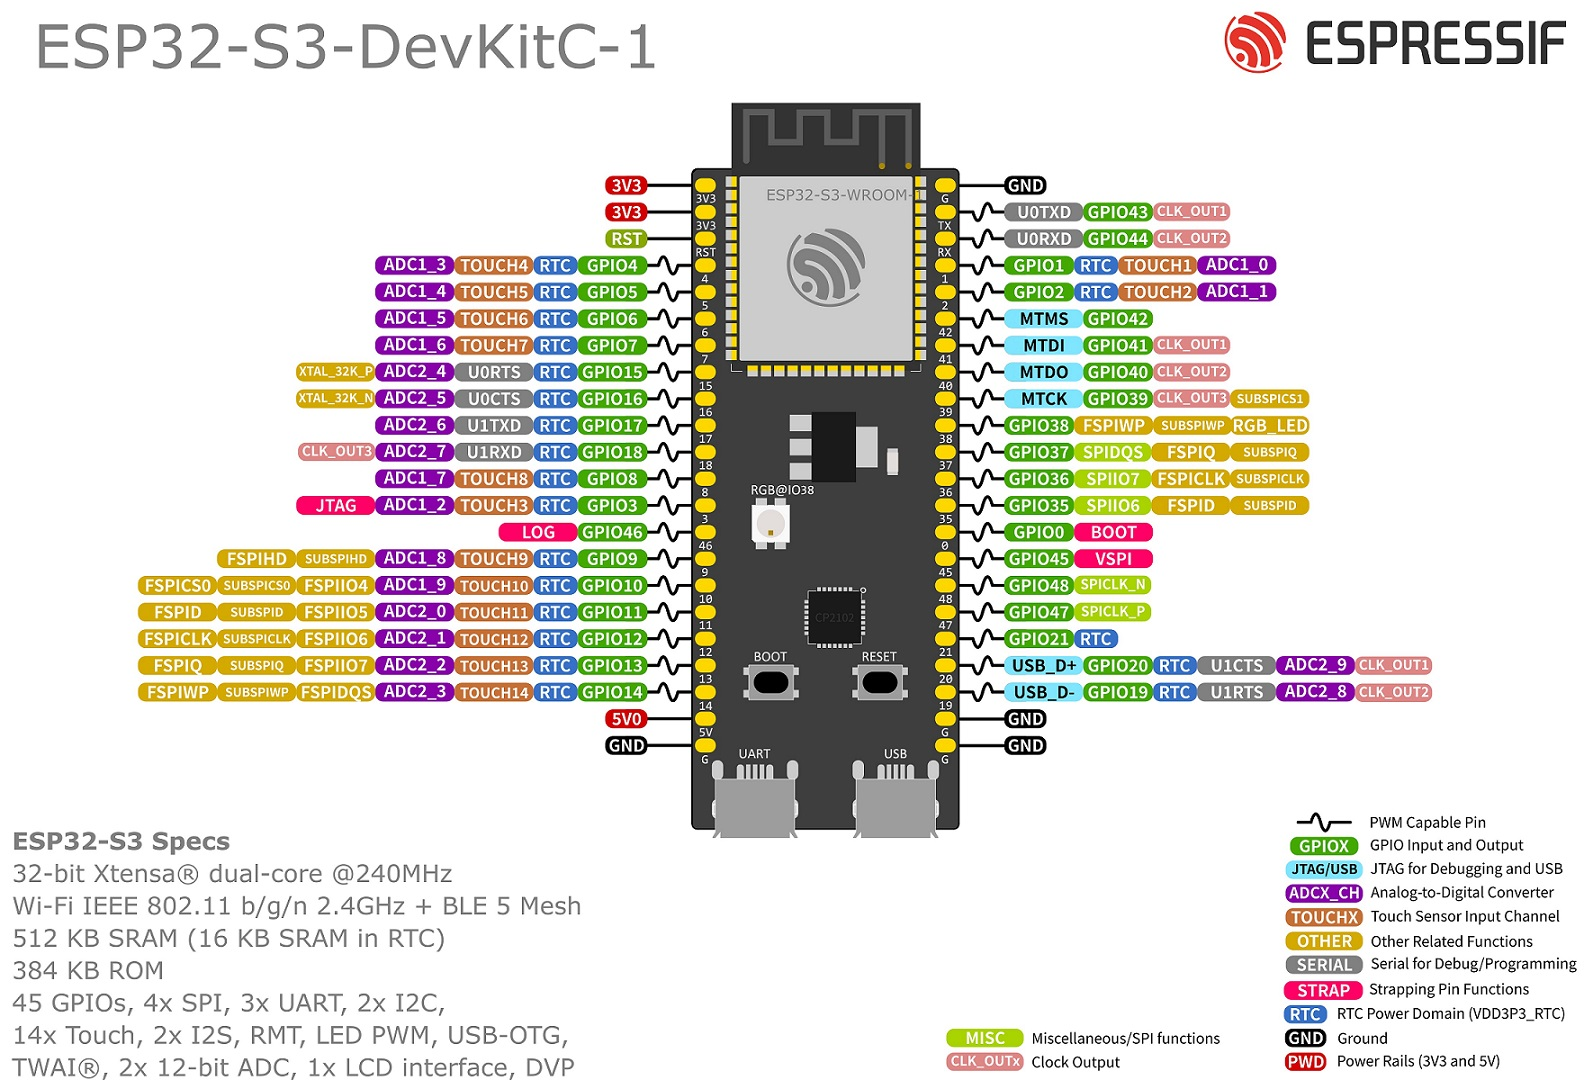
\includegraphics[width=1\textwidth]{./Images/ESP32-S3_DevKitC-1_pinlayout_v1.1.jpg}
    \caption{ESP32-S3 OBC Microcontroller}
    \label{fig:ESP32-S3}
\end{figure}

\subsection{Communications Subsystem}\label{communications_subsystem}

Communications are integral for the operations of this CubeSat system. Implemented within the system are 2 forms of inter-device communication. WiFi, being one of them, is included with both the ground station and OBC with the ground station being able to generate its own WiFi network that the OBC can connect to.

However, within CubeSat development WiFi is not the best analog for space communication. To give an alternative communication method more in line with a CubeSat a wireless RF transceiver module has been included with both the ground station and ORBITS unit.

The NRF24L01+, shown in figure \ref{fig:NRF24L01}, is a low cost, low power RF transceiver that fits the requirements needed by the ORBITS system. 
\begin{figure}[h]
    \centering
    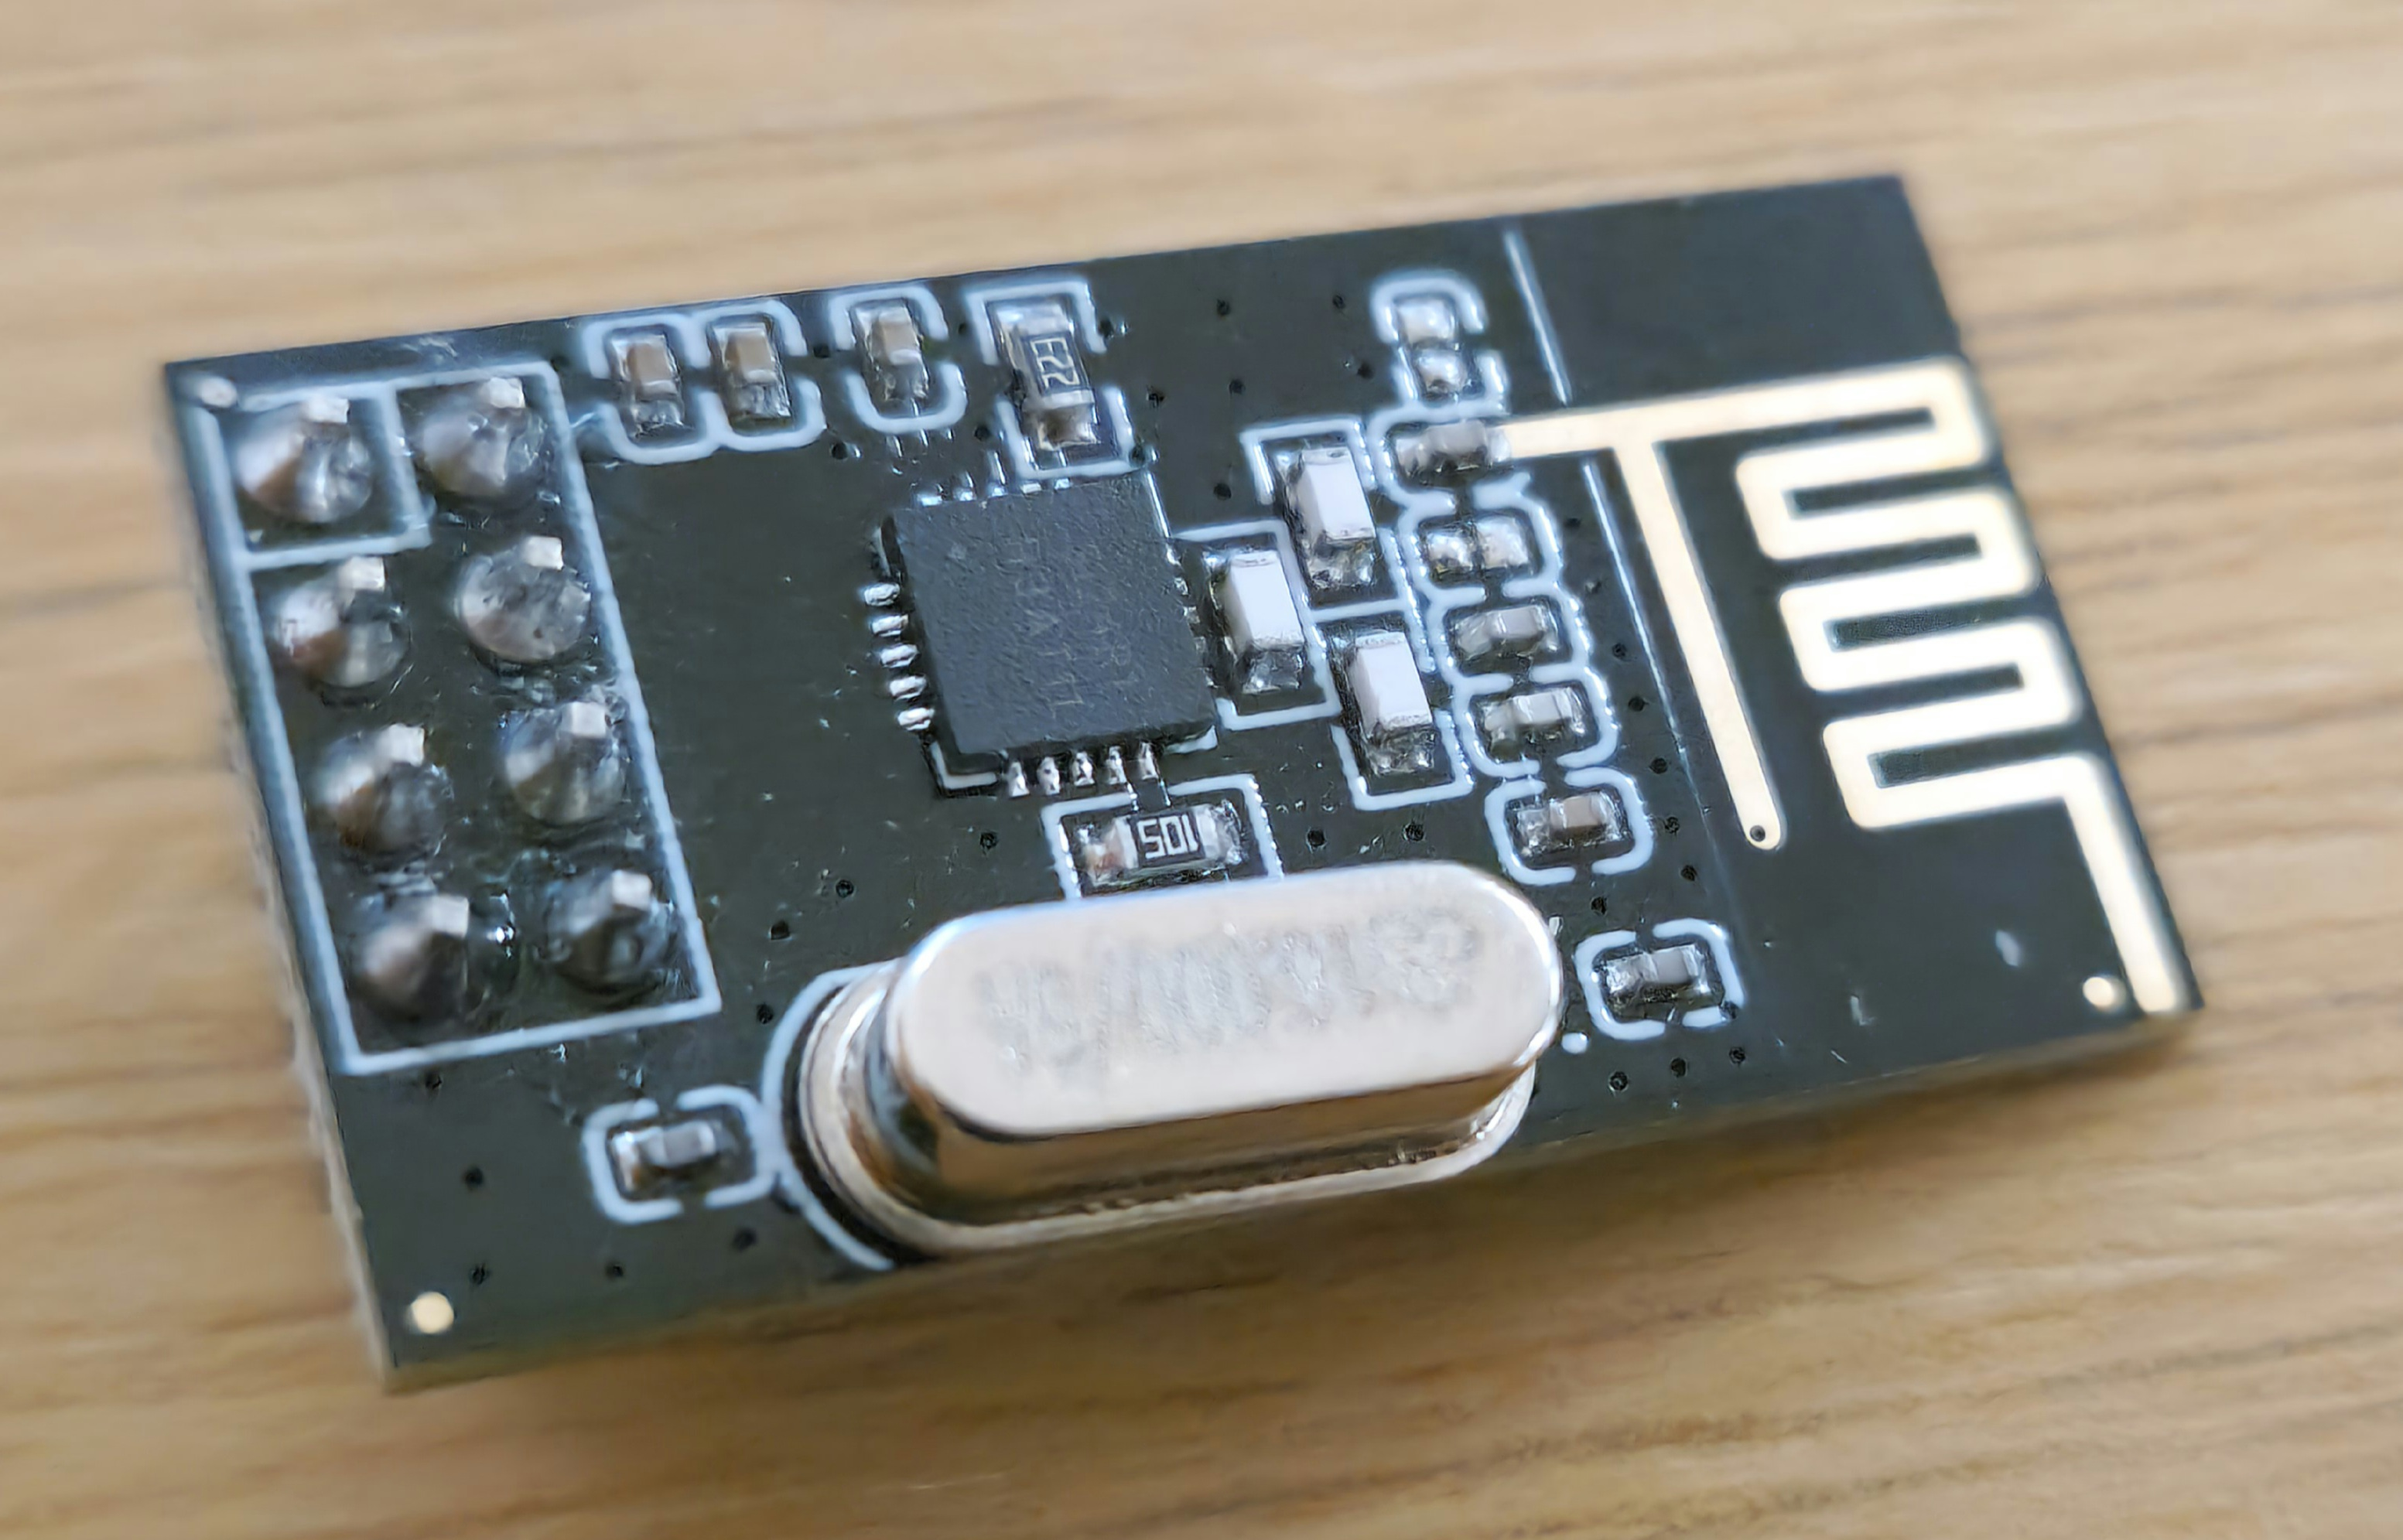
\includegraphics[width=0.5\textwidth]{./Images/NRF24L01.jpg}
    \caption{NRF24L01 RF Transceiver Module}
    \label{fig:NRF24L01}
\end{figure}
The 2.4GHz frequency band used by the module allows for easy communication without the need for a license. The NRF24L01 is able to achieve data rates of up to 2Mbps which is more than sufficient for the needs of the ORBITS system. The module also has a range of up to 100m in open space which is more than enough for a classroom environment. Due to the inexpensive nature of the module it has been widely used in the maker community and has a large ecosystem of learning materials and documentation which makes it an ideal choice for the ORBITS system.
\subsection{Power Management and Distribution Subsystem (PMAD)}

\subsection{Platform Structure}
\subsection{Attitude Determination and Control Subsystem (ADCS)}
\subsection{Payload}

\subsection{<Subsystem Name>}
\subsubsection{Purpose and Role}
<1--2 paragraphs describing what this subsystem does and why it is needed in ORBITS.>

\subsubsection{Selected Components}
\begin{table}[h]
\centering
\caption{Selected components for <Subsystem Name>}
\label{tab:<subsystem>_selected_components}
\begin{tabular}{|p{4cm}|p{4cm}|p{6cm}|}
\hline
\textbf{Component} & \textbf{Part Number} & \textbf{Key Specifications} \\ \hline
<e.g., MCU> & <e.g., ESP32-S3-N8R8-1U> & <clock, memory, IO, voltage, power> \\ \hline
<component 2> & <part number> & <key specs> \\ \hline
\end{tabular}
\end{table}

\subsubsection{Trade Study and Justification}
\begin{table}[h]
\centering
\caption{Trade study for <Subsystem Name>}
\label{tab:<subsystem>_trade_study}
\begin{tabular}{|p{3cm}|c|c|c|c|c|p{2.5cm}|}
\hline
\textbf{Option} & \textbf{Cost} & \textbf{Ecosystem} & \textbf{Performance} & \textbf{Avail.} & \textbf{P/P} & \textbf{Decision} \\ \hline
<Option A> & <1--5> & <1--5> & <1--5> & <1--5> & <1--5> & <Selected/Rejected> \\ \hline
<Option B> & <1--5> & <1--5> & <1--5> & <1--5> & <1--5> & <Selected/Rejected> \\ \hline
<Option C> & <1--5> & <1--5> & <1--5> & <1--5> & <1--5> & <Selected/Rejected> \\ \hline
\end{tabular}
\end{table}

\subsubsection{Interfaces and Integration}
\begin{itemize}
    \item \textbf{Electrical interface:} <voltage rails, max current, protection>
    \item \textbf{Data interface:} <UART/I2C/SPI/CAN/WiFi/NRF24L01, baud/data rate>
    \item \textbf{Mechanical interface:} <mounting, connector type, dimensions>
    \item \textbf{Software interface:} <driver/library, protocol, API boundary>
\end{itemize}

\subsubsection{Constraints, Risks, and Mitigations}
\begin{table}[h]
\centering
\caption{Risks for <Subsystem Name>}
\label{tab:<subsystem>_risks}
\begin{tabular}{|p{5cm}|p{3cm}|p{6cm}|}
\hline
\textbf{Risk} & \textbf{Impact/Likelihood} & \textbf{Mitigation} \\ \hline
<risk 1> & <H/M/L> & <mitigation action> \\ \hline
<risk 2> & <H/M/L> & <mitigation action> \\ \hline
\end{tabular}
\end{table}

\subsubsection{Verification and Validation Plan}
\begin{table}[h]
\centering
\caption{Verification plan for <Subsystem Name>}
\label{tab:<subsystem>_verification}
\begin{tabular}{|p{2cm}|p{5cm}|p{4cm}|p{3cm}|}
\hline
\textbf{Test ID} & \textbf{Requirement/Objective} & \textbf{Method} & \textbf{Pass Criteria} \\ \hline
T-<sub>-01 & <what must be proven> & <bench/simulation/field test> & <quantitative threshold> \\ \hline
T-<sub>-02 & <what must be proven> & <bench/simulation/field test> & <quantitative threshold> \\ \hline
\end{tabular}
\end{table}

\subsubsection{Summary}
<Short paragraph linking this subsystem back to system-level requirements.>

\section{Software Overview} \label{software_design}
\section{Learning Material}
Maybe an appendix with the learning materials and instructions for use of the system
\section{Bill of Materials}
Can probably be put in an appendix
\section{Software Documentation}
\printbibliography
\end{document}